\bibliographystyle{babplain-fl}

\chapter{Encontrar ceros de funciones}
\label{cha:ceros-funciones}

  Se habla de encontrar la \emph{raíz} de una ecuación:
  \begin{equation*}
    f(x)
      = 0
  \end{equation*}
  mientras se busca un \emph{cero} de la función \(f(x)\).
  El problema de hallar ceros de funciones es muy común.
  Lamentablemente solo en casos muy especiales hay fórmulas exactas,
  la mayor parte de las veces
  debe recurrirse a hallar buenas aproximaciones numéricas.
  Un buen resumen y ejemplos da Wright~%
    \cite{wright04:_nonlinear_root_finding}.
  Incluso se da el caso que hay soluciones exactas,
  pero la fórmula del caso es engorrosa
  (o tiene malas propiedades numéricas),
  resulta más cómodo
  e incluso más exacto usar una técnica iterativa.
  Una discusión detallada de algunas técnicas se hallan en las notas
  de LeMesurier y Roberts~%
    \cite{lemesurier97:_b15_numerical_analysis}.

  El problema es dada \(f(x)\),
  hallar \(x^*\) tal que \(f(x^*) = 0\)
  (\(f\) debe ser continua).
  Por ejemplo:
  ¿para qué valor de \(x\) se cumple \(x = e^{-x}\)?
  Una idea para resolver este problema es simplemente graficar la función.
  \begin{equation}
    f(x)
      = x - e^{-x}
  \end{equation}
  y ver cuáles son los valores de \(x^*\) tal que \(f(x^*) = 0\).
  \begin{figure}[ht]
    \centering
    \begin{tikzpicture}
      \begin{axis}[axis x line = middle, axis y line = left,
                   xlabel = {\(x\)}, ylabel ={\(f(x) = x - \mathrm{e}^{-x}\)},
                   xmin = 0, xmax = 2.3,
                   ymin = -1, ymax = 2.3]

        \addplot [mark = none, red] {x - exp(-x)};
      \end{axis}
    \end{tikzpicture}
    \caption{Gráfica de la función \(x - \mathrm{e}^{-x}\)}
    \label{fig:plot-f}
  \end{figure}
  En la figura~\ref{fig:plot-f} se aprecia un cero cerca de \num{0,6}.

  Otra forma de solucionar el problema
  puede ser graficar \(x\), \(e^{-x}\),
  para buscar las intersecciones
  (figura~\ref{fig:plot-intersect}).
  \begin{figure}[ht]
    \centering
    \begin{tikzpicture}
      \begin{axis}[axis lines = left,
                   xlabel = {\(x\)}, ylabel = {\(y\)},
                   xmin = 0, xmax = 1.1,
                   ymin = 0, ymax = 1.1]

        \addplot [mark = none, domain = 0:1, blue] {x};
        \addplot [mark = none, domain = 0:1, red] {exp(-x)};

        \draw[dashed, blue]
          (axis cs: 0.567143, 0) -- (axis cs: 0.567143, 0.567143);
      \end{axis}
    \end{tikzpicture}
    \caption{Gráficas de \(x\) y \(\mathrm{e}^{-x}\)}
    \label{fig:plot-intersect}
  \end{figure}

\section{Métodos que acotan el tramo}

  Corresponden a métodos para encontrar ceros de funciones
  los cuales usan el \emph{teorema del valor intermedio}
  y que básicamente van encerrando la solución
  hasta acotarla a un tramo suficientemente corto
  (en inglés, \emph{\foreignlanguage{english}{bracketing}}).
  Consideraremos dos métodos de este tipo:
  el método de la bisección y \foreignlanguage{latin}{\emph{regula falsi}}.

\subsection{Método de la Bisección}

  Si tenemos \(x_0, x_1\) tales que \(f(x_0)\cdot f(x_1) < 0\),
  hay un cero de \(f\) en \(\left[ x_0, x_1 \right]\),
  elegimos
  \begin{equation}
    x_2
      = \frac{x_0 + x_1}{2}
  \end{equation}
  con \(\left[ x_0, x_2\right]\) o \(\left[ x_2, x_1\right]\)
  según el cual tenga valores de \(f\) de signo distinto.
  \begin{figure}[ht]
    \centering
    \begin{tikzpicture}
      \begin{axis}[
                    axis lines = center,
                    xlabel = \(x\),
                    ylabel = {\(y = f(x)\)},
                    every axis y
                      label/.style = {at = (current axis.above origin),
                        anchor = south},
                    every axis x
                      label/.style = {at = (current axis.right of origin),
                        anchor = west},
                    xmin = 0,  xmax = 2,
                    ymin = -2, ymax = 2,
                    xtick = {0.3, 0.85, 1.4},
                    xticklabels = {\(x_0\), \(x_2\), \(x_1\)},
                    ytick = {0.8, -0.6},
                    yticklabels = {\(f(x_0)\), \(f(x_1)\)},
                    height = 6cm, width = 9cm
                  ]
        \addplot [samples = 100, smooth, tension = 0.8, red]
          coordinates {(0.3, 0.8) (0.5, 1.7) (0.8, 0.4) (1.1, 0.9)
                       (1.3, -1) (1.4, -0.6)};

        \draw [blue, dashed] (axis cs:0.3, 0) -- (axis cs:0.3, 0.8);
        \draw [blue, dashed] (axis cs:1.4, 0) -- (axis cs:1.4, -0.6);

        \draw [blue, dashed] (axis cs:0, -0.6) -- (axis cs:1.4, -0.6);
        \draw [blue, dashed] (axis cs:0, 0.8) -- (axis cs:0.3, 0.8);
      \end{axis}
    \end{tikzpicture}
    \caption{Si \(f(x_0) \cdot f(x_1) < 0\),
             hay \(x^* \in [x_0, x_1]\)
             donde \(f(x^*) = 0\).}
    \label{01::BiseccionEjemplo1}
  \end{figure}
  Por ejemplo,
  consideremos la figura~\ref{01::BiseccionEjemplo1}.
  Podemos apreciar
  que el intervalo \(\left[x_2, x_1\right]\)
  cumple con \(f(x_2)\cdot f(x_1)<0\).
  En consecuencia,
  por el teorema del valor intermedio
  sabemos que \(x^*\in\left[x_2, x_1\right]\).
  Luego,
  para aproximar \(x^*\)
  obtenemos el valor medio del intervalo \(\left[x_2, x_1\right]\)
  y repetimos el proceso.

  Note que la gracia de todo esto es encontrar solo \emph{un} cero,
  ¡no todos!
  Esto quiere decir lo ideal
  es escoger intervalo \([a, b]\) tal que solo tenga \emph{un} cero.
  Si nuestra función solo toca el eje \(X\)
  (vale decir,
   tiene un cero de multiplicidad par)
  esto claramente no sirve.
  Si hay varios ceros en el intervalo,
  convergerá a uno de ellos.
  \begin{figure}[ht]
    \centering
    \begin{tikzpicture}
      \begin{axis}[
                    axis lines = center,
                    xlabel = \(x\),
                    ylabel = {\(y = f(x)\)},
                    every axis y
                      label/.style = {at = (current axis.above origin),
                        anchor = south},
                    every axis x
                      label/.style = {at = (current axis.right of origin),
                        anchor = west},
                    xmin = 0,  xmax = 2,
                    ymin = -2, ymax = 2,
                    xtick = {0.3, 0.85, 1.4},
                    xticklabels = {\(x_0\), \(x_2\), \(x_1\)},
                    ytick = {0},
                    yticklabels = {},
                    height = 6cm, width = 9cm
                  ]
        \addplot [samples = 100, smooth, tension = 0.8, red]
          coordinates {(0.3, 0.8) (0.5, 1.7) (0.8, -0.9) (1.1, 0.9)
                       (1.3, -1) (1.4, -0.6)};

        \draw [blue, dashed] (axis cs:0.3, 0) -- (axis cs:0.3, 0.8);
        \draw [blue, dashed] (axis cs:1.4, 0) -- (axis cs:1.4, -0.6);
      \end{axis}
    \end{tikzpicture}
    \caption{Una función con tres ceros.}
    \label{01::BiseccionEjemplo2}
  \end{figure}
  Por lo tanto,
  el método de la bisección no abarca todos los casos posibles.

\subsection{Método \foreignlanguage{latin}{\emph{Regula Falsi}}}

  Siempre podemos usar la antigua idea
  (se traza a la antigua Babilonia)
  de tomar dos puntos que acoten un cero
  en la curva
  e interpolar linealmente para obtener una aproximación mejor,
  vea la figura~\ref{01::RegularFalsi:grafico}.
  Esto da:
  \begin{equation}
    \label{eq:regula-falsi-start}
    x_2
      = x_1 - f(x_1) \cdot \frac{x_1 - x_0}{f(x_1) - f(x_0)}
  \end{equation}
  \begin{figure}[ht]
    \centering
    % The function interpolates:
    % 0.2   0.9
    % 0.3   0.7
    % 0.9   0.0
    % 1.7  -0.3
    % 1.9  -0.35
    % see regula-falsi.mc
    \begin{tikzpicture}
      \begin{axis}[
                    axis lines = center,
                    xlabel = {\(x\)},
                    ylabel = {\(y\)},
                    every axis y
                      label/.style = {at = (current axis.above origin),
                        anchor = south},
                    every axis x
                      label/.style = {at = (current axis.right of origin),
                        anchor = west},
                    xmin = 0,	 xmax = 2,
                    ymin = -0.6, ymax = 1,
                    xtick = {3/10},
                    xticklabels = {\(x_0\)},
                    extra x ticks = {32/25, 17/10},
                    extra x tick labels = {\(x_2\), \(x_1\)},
                    extra x tick style = {
                      xticklabel style = {yshift = 0.5ex, anchor = south}
                    },
                    ytick = {0},
                    yticklabels = {},
                    height = 6cm, width = 9cm
                  ]
        \addplot [red, smooth, domain = 0.2:1.9]
          {(19000 * x^4 - 154100 * x^3 + 460190 * x^2 - 659011 * x + 320229)
             / 228480};
        \addplot [blue, samples = 100, domain = 0.3:1.7]
          {(32 - 25 * x) / 35};

        \draw [dashed, blue]
           (axis cs:3/10, 0) -- (axis cs:3/10, 7/10);
        \draw [dashed, blue]
           (axis cs:32/25, 0) -- (axis cs:32/25, -6175323/34000000);
        \draw [dashed, blue]
           (axis cs:17/10, 0) -- (axis cs:17/10, -3/10);
      \end{axis}
    \end{tikzpicture}
    \caption{\foreignlanguage{latin}{\emph{Regula falsi}}}
    \label{01::RegularFalsi:grafico}
  \end{figure}
  De allí procedemos iterando,
  calculando:
  \begin{equation}
    \label{eq:regula-falsi-iteration}
    x_{n + 1}
      = x_n - f(x_n) \cdot \frac{x_n - x_0}{f(x_n) - f(x_0)}
  \end{equation}
  Mantenemos fijo el punto inicial \(x_0\),
  la exigencia de siempre horquillar el cero
  llevará a esta situación una vez estemos suficientemente cerca del cero
  (vea la figura~\ref{01::RegularFalsi:grafico}).

\section{Iteración de Punto Fijo}

  En inglés,
  a esta técnica
  se le llama \emph{\foreignlanguage{english}{fixed point iteration}}
  y se abrevia FPI.
  \begin{definition}
    Sea \(g(x)\) una función.
    Un \emph{punto fijo} de \(g\)
    es \(x^*\) tal que \(x^* = g(x^*)\).
  \end{definition}
  Es natural buscar aproximar un punto fijo de \(g\)
  mediante el siguiente esquema:
  Elegir algún \(x_0\) adecuado,
  y luego calcular sucesivamente:
  \begin{equation*}
    x_{n + 1}
      = g(x_n)
  \end{equation*}
  Dependiendo del punto inicial \(x_0\) y de las características de \(g\)
  esto tendrá
  (o no)
  éxito.

  Encontrar un cero de una función por algún método de punto fijo
  consiste en reescribir:
  \begin{equation*}
    f(x)
      = 0
  \end{equation*}
  en la forma:
  \begin{equation*}
    g(x)
      = x
  \end{equation*}
  Note que siempre podemos escribir:
  \begin{equation*}
    g(x)
      = x - \alpha f(x)
  \end{equation*}
  Queda elegir un \(\alpha \ne 0\) adecuado\ldots
  \begin{ejemplo}
    Supongamos que queremos encontrar una solución a la ecuación:
    \begin{equation*}
      x - \mathrm{e}^{-x}
        = 0
    \end{equation*}
    Alternativas de funciones a que buscar punto fijo
    basadas en la ecuación propuesta son:
    \begin{align*}
      x
        &= \mathrm{e}^{-x} \\
      x
        &= - \ln x \\
      x
        &= x - \frac{2}{3} (x - \mathrm{e}^{-x})
    \end{align*}
    Como al crecer \(x\) aumenta \(x\)
    y disminuye (pero más lentamente) \(\mathrm{e}^{-x}\),
    la función dada es creciente,
    vemos que para \(x = 0\) es \(-1\)
    y para \(x = 1\) es \(1 - \mathrm{e}^{-1} > 0\),
    hay un cero en ese rango.
    Podemos elegir \(x_0 = 0,5\).
  \end{ejemplo}
  Usando iteraciones de punto fijo,
  se tiene que el cero de la función
  corresponde a la intersección entre \(y = x\) y \(g(x)\)
  (figura~\ref{01::FPI}).
  \begin{figure}[ht]
    \centering
    \begin{tikzpicture}
      \begin{axis}[
                    axis lines = center,
                    xlabel = {\(x\)},
                    ylabel = {\(y\)},
                    every axis y
                      label/.style = {at = (current axis.above origin),
                        anchor = south},
                    every axis x
                      label/.style = {at = (current axis.right of origin),
                        anchor = west},
                    xmin = 0, xmax = 2.5,
                    ymin = 0, ymax = 2,
                    xtick = {0.81},
                    xticklabels = {\(x^*\)},
                    ytick = {0},
                    yticklabels = {},
                    height = 6cm, width = 9cm
                  ]
        \addplot [domain = 0:1.4, blue]
           {x} node [yshift = 2pt, xshift = 13pt] (yx) {\(y = x\)};
        \addplot [domain = 0.5:1.6, red] {(1.5 - 0.7 * x)^3}
           node [yshift = 10pt] (g) {\(g(x)\)};

        \draw [dashed, blue] (axis cs:0.81, 0) -- (axis cs:0.81, 1.11);
      \end{axis}
    \end{tikzpicture}
    \caption{La intersección entre \(y = x\)
             e \(y = g(x)\) es un punto fijo}
    \label{01::FPI}
  \end{figure}
  Gráficamente,
  la iteración puede representarse en un gráfico de \(y = g(x)\)
  y la recta \(y = x\),
  el punto fijo es la intersección entre ambas.
  Partiendo del valor \(x_0\), calculamos \(g(x_0)\),
  lo que corresponde a ir en vertical a la curva para \(g\).
  Este valor será \(x_1\),
  cosa que corresponde a ir horizontalmente a la línea \(y = x\),
  dando la intersección como \(x_1\).
  Se puede ver como una espiral si \(g(x)\) es decreciente
  (figura~\ref{01::Espiral:convergente}
   y figura~\ref{01::Espiral:divergente}).
  \begin{figure}[ht]
    \centering
    % Ver cobweb-2.mc, cobwebs.raku para detalles
    \begin{tikzpicture}
      \begin{axis}[domain = 0:1,
                   axis x line = bottom, axis y line = left,
                   xmin = 0, xmax = 1,
                   ymin = 0, ymax = 1,
                   xtick = {0.1, 0.812, 0.25930573, 0.7084739004713133,
                     0.3257801870289462, 0.6545450715920982,
                     0.36698903565963403, 0.5},
                   xticklabels = {\(x_0^{\phantom{\ast}}\),
                                  \(x_1^{\phantom{\ast}}\),
                                  \(x_2^{\phantom{\ast}}\),
                                  \(x_3^{\phantom{\ast}}\),
                                  \(x_4^{\phantom{\ast}}\),
                                  \(\),
                                  \(\),
                                  \(x^{\ast}_{\phantom{0}}\)},
                   ytick style = {draw = none},
                   yticklabels = {}]

        \addplot[mark = none, blue] {x};
        \addplot[mark = none, red]
          {1 * x^3 / 1 - 7 * x^2 / 5 - 1 * x / 4 + 17 / 20};

      \draw [blue, very thin, dashed]
         (axis cs:0.1, 0) -- (axis cs:0.1, 0.812);
      \draw [blue, very thin, dashed]
         (axis cs:0.1, 0.812) -- (axis cs:0.812, 0.812);
      \draw [blue, very thin, dashed]
         (axis cs:0.812, 0.812) -- (axis cs:0.812, 0.25930573);
      \draw [blue, very thin, dashed]
         (axis cs:0.812, 0.25930573) -- (axis cs:0.25930573, 0.25930573);
      \draw [blue, very thin, dashed]
         (axis cs:0.25930573, 0.25930573)
              -- (axis cs:0.25930573, 0.7084739004713133);
      \draw [blue, very thin, dashed]
         (axis cs:0.25930573, 0.25930573)
              -- (axis cs:0.25930573, 0.7084739004713133);
      \draw [blue, very thin, dashed]
         (axis cs:0.25930573, 0.7084739004713133)
              -- (axis cs:0.7084739004713133, 0.7084739004713133);
      \draw [blue, very thin, dashed]
         (axis cs:0.7084739004713133, 0.7084739004713133)
              -- (axis cs:0.7084739004713133, 0.3257801870289462);
      \draw [blue, very thin, dashed]
         (axis cs:0.7084739004713133, 0.7084739004713133)
              -- (axis cs:0.7084739004713133, 0.3257801870289462);
      \draw [blue, very thin, dashed]
         (axis cs:0.7084739004713133, 0.3257801870289462)
              -- (axis cs:0.3257801870289462, 0.3257801870289462);
      \draw [blue, very thin, dashed]
         (axis cs:0.3257801870289462, 0.3257801870289462)
              -- (axis cs:0.3257801870289462, 0.6545450715920982);
      \draw [blue, very thin, dashed]
         (axis cs:0.3257801870289462, 0.3257801870289462)
              -- (axis cs:0.3257801870289462, 0.6545450715920982);
      \draw [blue, very thin, dashed]
         (axis cs:0.3257801870289462, 0.6545450715920982)
              -- (axis cs:0.6545450715920982, 0.6545450715920982);
      \draw [blue, very thin, dashed]
         (axis cs:0.6545450715920982, 0.6545450715920982)
              -- (axis cs:0.6545450715920982, 0.36698903565963403);
      \draw [blue, very thin, dashed]
         (axis cs:0.6545450715920982, 0.36698903565963403)
              -- (axis cs:0.36698903565963403, 0.36698903565963403);
      \end{axis}
    \end{tikzpicture}
    \caption{En este caso la espiral de iteración de punto fijo converge}
    \label{01::Espiral:convergente}
  \end{figure}
  \begin{figure}[ht]
    \centering
    % Ver cobweb-1.mc, cobwebs.raku para detalles
    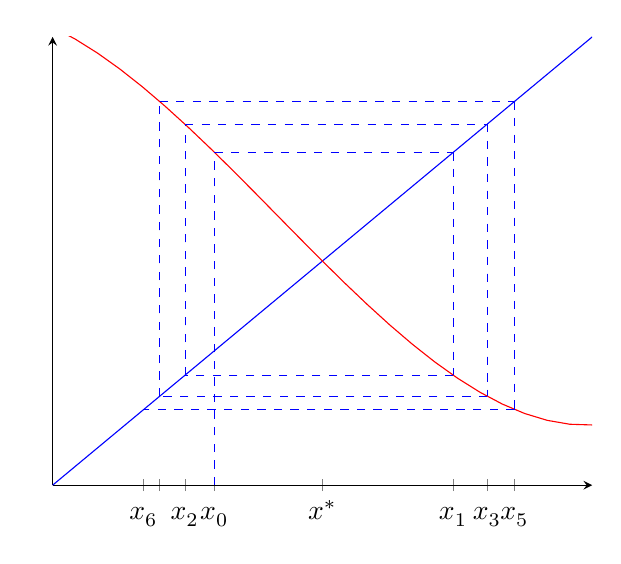
\begin{tikzpicture}
      \begin{axis}[domain = 0:1,
                   axis x line = bottom, axis y line = left,
                   xmin = 0, xmax = 1,
                   ymin = 0, ymax = 1,
                   xtick = {0.3, 0.7425, 0.245202598, 0.8053675633204307,
                     0.19829350349601982, 0.8561644490113705,
                     0.1687199716882174, 0.5},
                   xticklabels = {\(x_0^{\phantom{\ast}}\),
                                  \(x_1^{\phantom{\ast}}\),
                                  \(x_2^{\phantom{\ast}}\),
                                  \(x_3^{\phantom{\ast}}\),
                                  \(\),
                                  \(x_5^{\phantom{\ast}}\),
                                  \(x_6^{\phantom{\ast}}\),
                                  \(x^{\ast}_{\phantom{0}}\)},
                   ytick style = {draw = none},
                   yticklabels = {}]

        \addplot[mark = none, blue] {x};
        \addplot[mark = none, red]
          {5 * x^3 / 4 - 25 * x^2 / 16 - 23 * x / 40 + 327 / 320};

      \draw [blue, very thin, dashed]
         (axis cs:0.3, 0) -- (axis cs:0.3, 0.7425);
      \draw [blue, very thin, dashed]
         (axis cs:0.3, 0.7425) -- (axis cs:0.7425, 0.7425);
      \draw [blue, very thin, dashed]
         (axis cs:0.7425, 0.7425) -- (axis cs:0.7425, 0.245202598);
      \draw [blue, very thin, dashed]
         (axis cs:0.7425, 0.245202598) -- (axis cs:0.245202598, 0.245202598);
      \draw [blue, very thin, dashed]
         (axis cs:0.245202598, 0.245202598)
             -- (axis cs:0.245202598, 0.8053675633204307);
      \draw [blue, very thin, dashed]
         (axis cs:0.245202598, 0.245202598)
             -- (axis cs:0.245202598, 0.8053675633204307);
      \draw [blue, very thin, dashed]
      (axis cs:0.245202598, 0.8053675633204307)
             -- (axis cs:0.8053675633204307, 0.8053675633204307);
      \draw [blue, very thin, dashed]
         (axis cs:0.8053675633204307, 0.8053675633204307)
             -- (axis cs:0.8053675633204307, 0.19829350349601982);
      \draw [blue, very thin, dashed]
         (axis cs:0.8053675633204307, 0.8053675633204307)
             -- (axis cs:0.8053675633204307, 0.19829350349601982);
      \draw [blue, very thin, dashed]
         (axis cs:0.8053675633204307, 0.19829350349601982)
             -- (axis cs:0.19829350349601982, 0.19829350349601982);
      \draw [blue, very thin, dashed]
         (axis cs:0.19829350349601982, 0.19829350349601982)
             -- (axis cs:0.19829350349601982, 0.8561644490113705);
      \draw [blue, very thin, dashed]
         (axis cs:0.19829350349601982, 0.19829350349601982)
              -- (axis cs:0.19829350349601982, 0.8561644490113705);
      \draw [blue, very thin, dashed]
         (axis cs:0.19829350349601982, 0.8561644490113705)
              -- (axis cs:0.8561644490113705, 0.8561644490113705);
      \draw [blue, very thin, dashed]
         (axis cs:0.8561644490113705, 0.8561644490113705)
              -- (axis cs:0.8561644490113705, 0.1687199716882174);
      \draw [blue, very thin, dashed]
         (axis cs:0.8561644490113705, 0.1687199716882174)
              -- (axis cs:0.1687199716882174, 0.1687199716882174);
      \end{axis}
    \end{tikzpicture}
    \caption{En este caso la espiral de iteración de punto fijo diverge}
    \label{01::Espiral:divergente}
  \end{figure}
  A los diagramas de las figuras~\ref{01::Espiral:convergente}
  y~\ref{01::Espiral:divergente}
  les llaman \emph{diagrama de telaraña}
  (en inglés,
   \emph{\foreignlanguage{english}{cobweb diagram}})
  por razones fáciles de ver.
  Note que para construir estas espirales
  debe partir por el eje \(x\),
  en algún \(x_0\) a su gusto.
  Luego,
  tirar una línea vertical hasta chocar con \(g\).
  En seguida,
  continúe con una línea horizontal hasta llegar a \(y = x\)
  y vuelva a trazar otra vertical hasta \(g(x)\).
  Continúe así hasta encontrar una aproximación suficiente
  al punto fijo.

  Las figuras~\ref{01::Espiral:convergente} y~\ref{01::Espiral:divergente}
  ilustran que si \(g(x)\) es decreciente en el rango de interés
  y la gráfica de \(y = g(x)\) se acerca a la horizontal
  cerca del punto de intersección con \(y = x\),
  el método converge.
  En cambio,
  si la gráfica de \(y = g(x)\) se acerca a la vertical,
  diverge.

  En caso que \(g\) sea creciente en vez de una espiral
  se obtiene una escalera,
  vea las figuras~\ref{fig:FIP-increasing-converges}
  y~\ref{fig:FIP-increasing-diverges}.
  \begin{figure}
    \centering
    % Ver cobweb-4.mc, cobwebs.raku para detalles
    \begin{tikzpicture}
      \begin{axis}[domain = 0:1,
                   axis x line = bottom, axis y line = left,
                   xmin = 0, xmax = 1,
                   ymin = 0, ymax = 1,
                   xtick = {0.1, 0.5000066, 0.678700259368431587,
                     0.7312996515938205, 0.74701294446039,
                     0.7518459248664618, 0.7533485113148211, 0.75},
                   xticklabels = {\(x_0^{\phantom{\ast}}\),
                                  \(x_1^{\phantom{\ast}}\),
                                  \(x_2^{\phantom{\ast}}\),
                                  \(\),
                                  \(\),
                                  \(\),
                                  \(\),
                                  \(x^{\ast}_{\phantom{0}}\)},
                   ytick style = {draw = none},
                   yticklabels = {}]

        \addplot[mark = none, blue] {x};
        \addplot[mark = none, red]
                {680 * x^3 / 1521 - 1270 * x^2 / 1521
                  + 16409 * x / 20280 + 5773 / 13520};

      \draw [blue, very thin, dashed]
         (axis cs:0.1, 0) -- (axis cs:0.1, 0.5000066);
      \draw [blue, very thin, dashed]
         (axis cs:0.1, 0.5000066) -- (axis cs:0.5000066, 0.5000066);
      \draw [blue, very thin, dashed]
         (axis cs:0.5000066, 0.5000066)
              -- (axis cs:0.5000066, 0.678700259368431587);
      \draw [blue, very thin, dashed]
         (axis cs:0.5000066, 0.678700259368431587)
              -- (axis cs:0.678700259368431587, 0.678700259368431587);
      \draw [blue, very thin, dashed]
         (axis cs:0.678700259368431587, 0.678700259368431587)
              -- (axis cs:0.678700259368431587, 0.7312996515938205);
      \draw [blue, very thin, dashed]
         (axis cs:0.678700259368431587, 0.678700259368431587)
              -- (axis cs:0.678700259368431587, 0.7312996515938205);
      \draw [blue, very thin, dashed]
         (axis cs:0.678700259368431587, 0.7312996515938205)
              -- (axis cs:0.7312996515938205, 0.7312996515938205);
      \draw [blue, very thin, dashed]
         (axis cs:0.7312996515938205, 0.7312996515938205)
              -- (axis cs:0.7312996515938205, 0.74701294446039);
      \draw [blue, very thin, dashed]
         (axis cs:0.7312996515938205, 0.7312996515938205)
              -- (axis cs:0.7312996515938205, 0.74701294446039);
      \draw [blue, very thin, dashed]
         (axis cs:0.7312996515938205, 0.74701294446039)
              -- (axis cs:0.74701294446039, 0.74701294446039);
      \draw [blue, very thin, dashed]
         (axis cs:0.74701294446039, 0.74701294446039)
              -- (axis cs:0.74701294446039, 0.7518459248664618);
      \draw [blue, very thin, dashed]
         (axis cs:0.74701294446039, 0.74701294446039)
              -- (axis cs:0.74701294446039, 0.7518459248664618);
      \draw [blue, very thin, dashed]
         (axis cs:0.74701294446039, 0.7518459248664618)
              -- (axis cs:0.7518459248664618, 0.7518459248664618);
      \draw [blue, very thin, dashed]
         (axis cs:0.7518459248664618, 0.7518459248664618)
              -- (axis cs:0.7518459248664618, 0.7533485113148211);
      \draw [blue, very thin, dashed]
         (axis cs:0.7518459248664618, 0.7533485113148211)
              -- (axis cs:0.7533485113148211, 0.7533485113148211);
      \end{axis}
    \end{tikzpicture}
    \caption{La escalera de iteración de punto fijo converge}
    \label{fig:FIP-increasing-converges}
  \end{figure}
  \begin{figure}
    \centering
    % Ver cobweb-3.mc, cobwebs.raku para detalles
    \begin{tikzpicture}
      \begin{axis}[domain = 0:1,
                   axis x line = bottom, axis y line = left,
                   xmin = 0, xmax = 1,
                   ymin = 0, ymax = 1,
                   xtick = {0.3, 0.323028, 0.355531714912121,
                     0.40050722374171244, 0.4615564206393762,
                     0.5436710682749981, 0.6563153774050898, 0.25},
                   xticklabels = {\(x_0^{\phantom{\ast}}\),
                                  \(\),
                                  \(\),
                                  \(x_3^{\phantom{\ast}}\),
                                  \(x_4^{\phantom{\ast}}\),
                                  \(x_5^{\phantom{\ast}}\),
                                  \(x_6^{\phantom{\ast}}\),
                                  \(x^{\ast}_{\phantom{0}}\)},
                   ytick style = {draw = none},
                   yticklabels = {}]

        \addplot[mark = none, blue] {x};
        \addplot[mark = none, red]
                {2450 * x^3 / 1521 - 3160 * x^2 / 1521 + 27217 * x / 12168
                  - 553 / 2704};

      \draw [blue, very thin, dashed]
         (axis cs:0.3, 0) -- (axis cs:0.3, 0.323028);
      \draw [blue, very thin, dashed]
         (axis cs:0.3, 0.323028) -- (axis cs:0.323028, 0.323028);
      \draw [blue, very thin, dashed]
         (axis cs:0.323028, 0.323028) -- (axis cs:0.323028, 0.355531714912121);
      \draw [blue, very thin, dashed]
         (axis cs:0.323028, 0.355531714912121)
              -- (axis cs:0.355531714912121, 0.355531714912121);
      \draw [blue, very thin, dashed]
         (axis cs:0.355531714912121, 0.355531714912121)
              -- (axis cs:0.355531714912121, 0.40050722374171244);
      \draw [blue, very thin, dashed]
         (axis cs:0.355531714912121, 0.355531714912121)
              -- (axis cs:0.355531714912121, 0.40050722374171244);
      \draw [blue, very thin, dashed]
         (axis cs:0.355531714912121, 0.40050722374171244)
              -- (axis cs:0.40050722374171244, 0.40050722374171244);
      \draw [blue, very thin, dashed]
         (axis cs:0.40050722374171244, 0.40050722374171244)
              -- (axis cs:0.40050722374171244, 0.4615564206393762);
      \draw [blue, very thin, dashed]
         (axis cs:0.40050722374171244, 0.40050722374171244)
              -- (axis cs:0.40050722374171244, 0.4615564206393762);
      \draw [blue, very thin, dashed]
         (axis cs:0.40050722374171244, 0.4615564206393762)
              -- (axis cs:0.4615564206393762, 0.4615564206393762);
      \draw [blue, very thin, dashed]
         (axis cs:0.4615564206393762, 0.4615564206393762)
              -- (axis cs:0.4615564206393762, 0.5436710682749981);
      \draw [blue, very thin, dashed]
         (axis cs:0.4615564206393762, 0.4615564206393762)
              -- (axis cs:0.4615564206393762, 0.5436710682749981);
      \draw [blue, very thin, dashed]
         (axis cs:0.4615564206393762, 0.5436710682749981)
              -- (axis cs:0.5436710682749981, 0.5436710682749981);
      \draw [blue, very thin, dashed]
         (axis cs:0.5436710682749981, 0.5436710682749981)
              -- (axis cs:0.5436710682749981, 0.6563153774050898);
      \draw [blue, very thin, dashed]
         (axis cs:0.5436710682749981, 0.6563153774050898)
              -- (axis cs:0.6563153774050898, 0.6563153774050898);
      \end{axis}
    \end{tikzpicture}
    \caption{La escalera de iteración de punto fijo diverge}
    \label{fig:FIP-increasing-diverges}
  \end{figure}


\subsection{Método de la Secante}

  La idea,
  al igual que para \foreignlanguage{latin}{\emph{regula falsi}},
  es calcular el intercepto de la recta que pasa por dos puntos,
  ver figura~\ref{01::secante:grafico}.
  Pero a diferencia de ese método,
  no se mantienen puntos fijos.
  Partiendo con \(x_0, x_1\)
  se calculan valores sucesivos
  usando:
  \begin{equation*}
    x_{n + 2}
      = x_{n + 1}
          - f(x_{n + 1}) \cdot \frac{x_{n + 1} - x_n}{f(x_{n + 1}) - f(x_n)}
  \end{equation*}
  \begin{figure}[ht]
    \centering
    % The function interpolates:
    % 0.05  0.80
    % 0.15  0.40
    % 0.30  0.15
    % 0.40  0.00
    % 0.80 -0.30
    % See function.mc
    \begin{tikzpicture}
      \begin{axis}[
                    axis lines = center,
                    xlabel = {\(x\)},
                    ylabel = {\(y\)},
                    every axis y
                      label/.style = {at = (current axis.above origin),
                        anchor = south},
                    every axis x
                      label/.style = {at = (current axis.right of origin),
                        anchor = west},
                    xmin = 0,	 xmax = 0.5,
                    ymin = -0.6, ymax = 1.2,
                    xtick = {1/20, 3/10, 93/260},
                    xticklabels = {\small \(x_0\),
                                   \small \(x_1\),
                                   \small \(x_2\)},
                    ytick = {0},
                    yticklabels = {},
                    height = 6cm, width = 9cm
                  ]
        \addplot [blue]
           {(93 - 260 * x) / 100};
        \addplot [domain = 0.01:0.5, red]
           {(4740000 * x^4 - 7646000 * x^3 + 4231950 * x^2
              - 1167595 * x + 157926) / 136500};

        \draw [dashed, blue] (axis cs:1/20, 0) -- (axis cs:1/20, 4/5);
        \draw [dashed, blue] (axis cs:3/10, 0) -- (axis cs:3/10, 3/20);
      \end{axis}
    \end{tikzpicture}
    \caption{Una iteración del método de la secante.}
    \label{01::secante:grafico}
  \end{figure}
  La ventaja es que al usar puntos cada vez más cerca del cero
  la aproximación lineal se hace más precisa.
  Lo malo es que no asegura un rango que contiene el cero.

\subsection{Método de la tangente (Newton)}

  La idea consiste en elegir un valor arbitrario \(x_0\)
  que esté razonablemente cerca de \(x^*\) (cero de la función).
  Luego,
  sucesivamente encontramos el intercepto con el eje \(x\)
  de la recta tangente de la curva en \(x_n\) usando la ecuación:
  \begin{equation}\label{01::ecuacion:newton}
    x_{n + 1}
      = x_n - \frac{f(x_n)}{f'(x_n)}
  \end{equation}
  resultando un valor \(x_{n + 1}\)
  que se encuentra más cerca de \(x^*\) (figura~\ref{01::newton:grafico}).
  Finalmente,
  iteramos el proceso
  hasta obtener un valor suficientemente cercano al buscado.
  \begin{figure}[ht]
    \centering
    % The function interpolates:
    % 0.05  0.80
    % 0.15  0.40
    % 0.30  0.15
    % 0.40  0.00
    % 0.80 -0.30
    % See function.mc
    \begin{tikzpicture}
      \begin{axis}[
                    axis lines = center,
                    xlabel = {\(x\)},
                    ylabel = {\(y\)},
                    every axis y
                      label/.style = {at = (current axis.above origin),
                        anchor = south},
                    every axis x
                      label/.style = {at = (current axis.right of origin),
                        anchor = west},
                    xmin =  0,	 xmax = 0.5,
                    ymin = -0.6, ymax = 1.2,
                    xtick	= {3/20,    17139/56020},
                    xticklabels = {\small \(x_0\),
                                   \small \(x_1\)},
                    ytick = {0},
                    yticklabels = {},
                    height = 6cm, width = 9cm
                  ]
        \addplot [blue]
          {(17139 - 56020 * x) / 21480};
        \addplot [domain = 0.01:0.5, red]
           {(4740000 * x^4 - 7646000 * x^3 + 4231950 * x^2
              - 1167595 * x + 157926) / 136500};
        \draw [dashed, blue] (axis cs:3/20, 0) -- (axis cs:3/20, 2/5);
      \end{axis}
    \end{tikzpicture}
    \caption{El valor \(x_1\)
             de~\eqref{01::ecuacion:newton}
             es más cercano a \(x^*\) que \(x_0\).}
     \label{01::newton:grafico}
   \end{figure}

\section{Criterios de término}
\label{sec:stopping-criteria}

  Un tema pendiente es bajo qué condiciones terminar la iteración.
  Si el cero \(x^*\) es grande,
  basta asegurar que el error absoluto es pequeño;
  si es pequeño,
  es más relevante el error relativo.
  El criterio más robusto es exigir que se cumplan ambos.

  Pero desconocemos \(x^*\),
  tenemos que usar aproximaciones o algún esquema indirecto.
  En métodos que acotan el cero
  (como bisección),
  eso es relativamente simple.
  Detectar que nuestro método se comporta mal,
  o estamos cerca de los límites impuestos por errores de redondeo,
  no es fácil.
  Vea por ejemplo la discusión de Kahan del esquema iterativo de Cauchy~%
    \cite{kahan10:_estim_error_bound_cauchy_iteration}
  o sus notas sobre hallar ceros~%
    \cite{kahan16:_lecture_notes_real_root_finding}.

\section*{Ejercicios}
\label{sec:ejercicios-01}

  \begin{enumerate}
  \item
    Complete el ejemplo de aproximar el cero de \(x - \mathrm{e}^{-x}\)
    mediante iteración de punto fijo
    usando las alternativas de función con punto fijo planteadas.
    Ejecute algunas iteraciones y compare sus evoluciones.
  \item
    Usando nuevamente la ecuación \(x - \mathrm{e}^{-x}\),
    compare los métodos de bisección
    y \emph{\foreignlanguage{latin}{regula falsi}}
    con rango inicial \([0, 1]\).
    Compare el número de iteraciones necesarias
    para obtener cinco cifras significativas.
  \item
    Usando nuevamente la ecuación \(x - \mathrm{e}^{-x}\),
    compare los métodos de la secante
    (elija valores iniciales \(x_0 = 0\) y \(x_1 = 1\))
    y de Newton con valor inicial \(x_0 = 0\).
  \end{enumerate}

\bibliography{../referencias}

%%% Local Variables:
%%% mode: latex
%%% TeX-master: "../INF-221_notas"
%%% ispell-local-dictionary: "spanish"
%%% End:

% LocalWords:  recurrirse english bracketing latin falsi fixed point
% LocalWords:  iteration FPI cobweb diagram
